\documentclass[11pt, letterpaper]{article}
\usepackage[margin=1in]{geometry}
\usepackage{amsfonts}  %fonts like \mathbb{}
\usepackage{amssymb,amsmath}
\usepackage{graphicx}
\usepackage{mathrsfs} %for \mathscr

\title{Lectures on General Relativity}
\author{Juan Guarin, Antonio Calixto}
\date{August, 2023}

\def\Re{\mathbb{R}}

\begin{document}
%\maketitle
\begin{center}
	\huge \textbf{Lectures on General Relativity}
	
	\vspace{5mm}
	By: Juan Andrés Guarín-Rojas,\\
	Antonio Calixto Gutiérrez-Piñeres
	
	\vspace{5mm}
	August 30th, 2023
\end{center}
\vfill
\begin{figure}[hb]
	\centering
	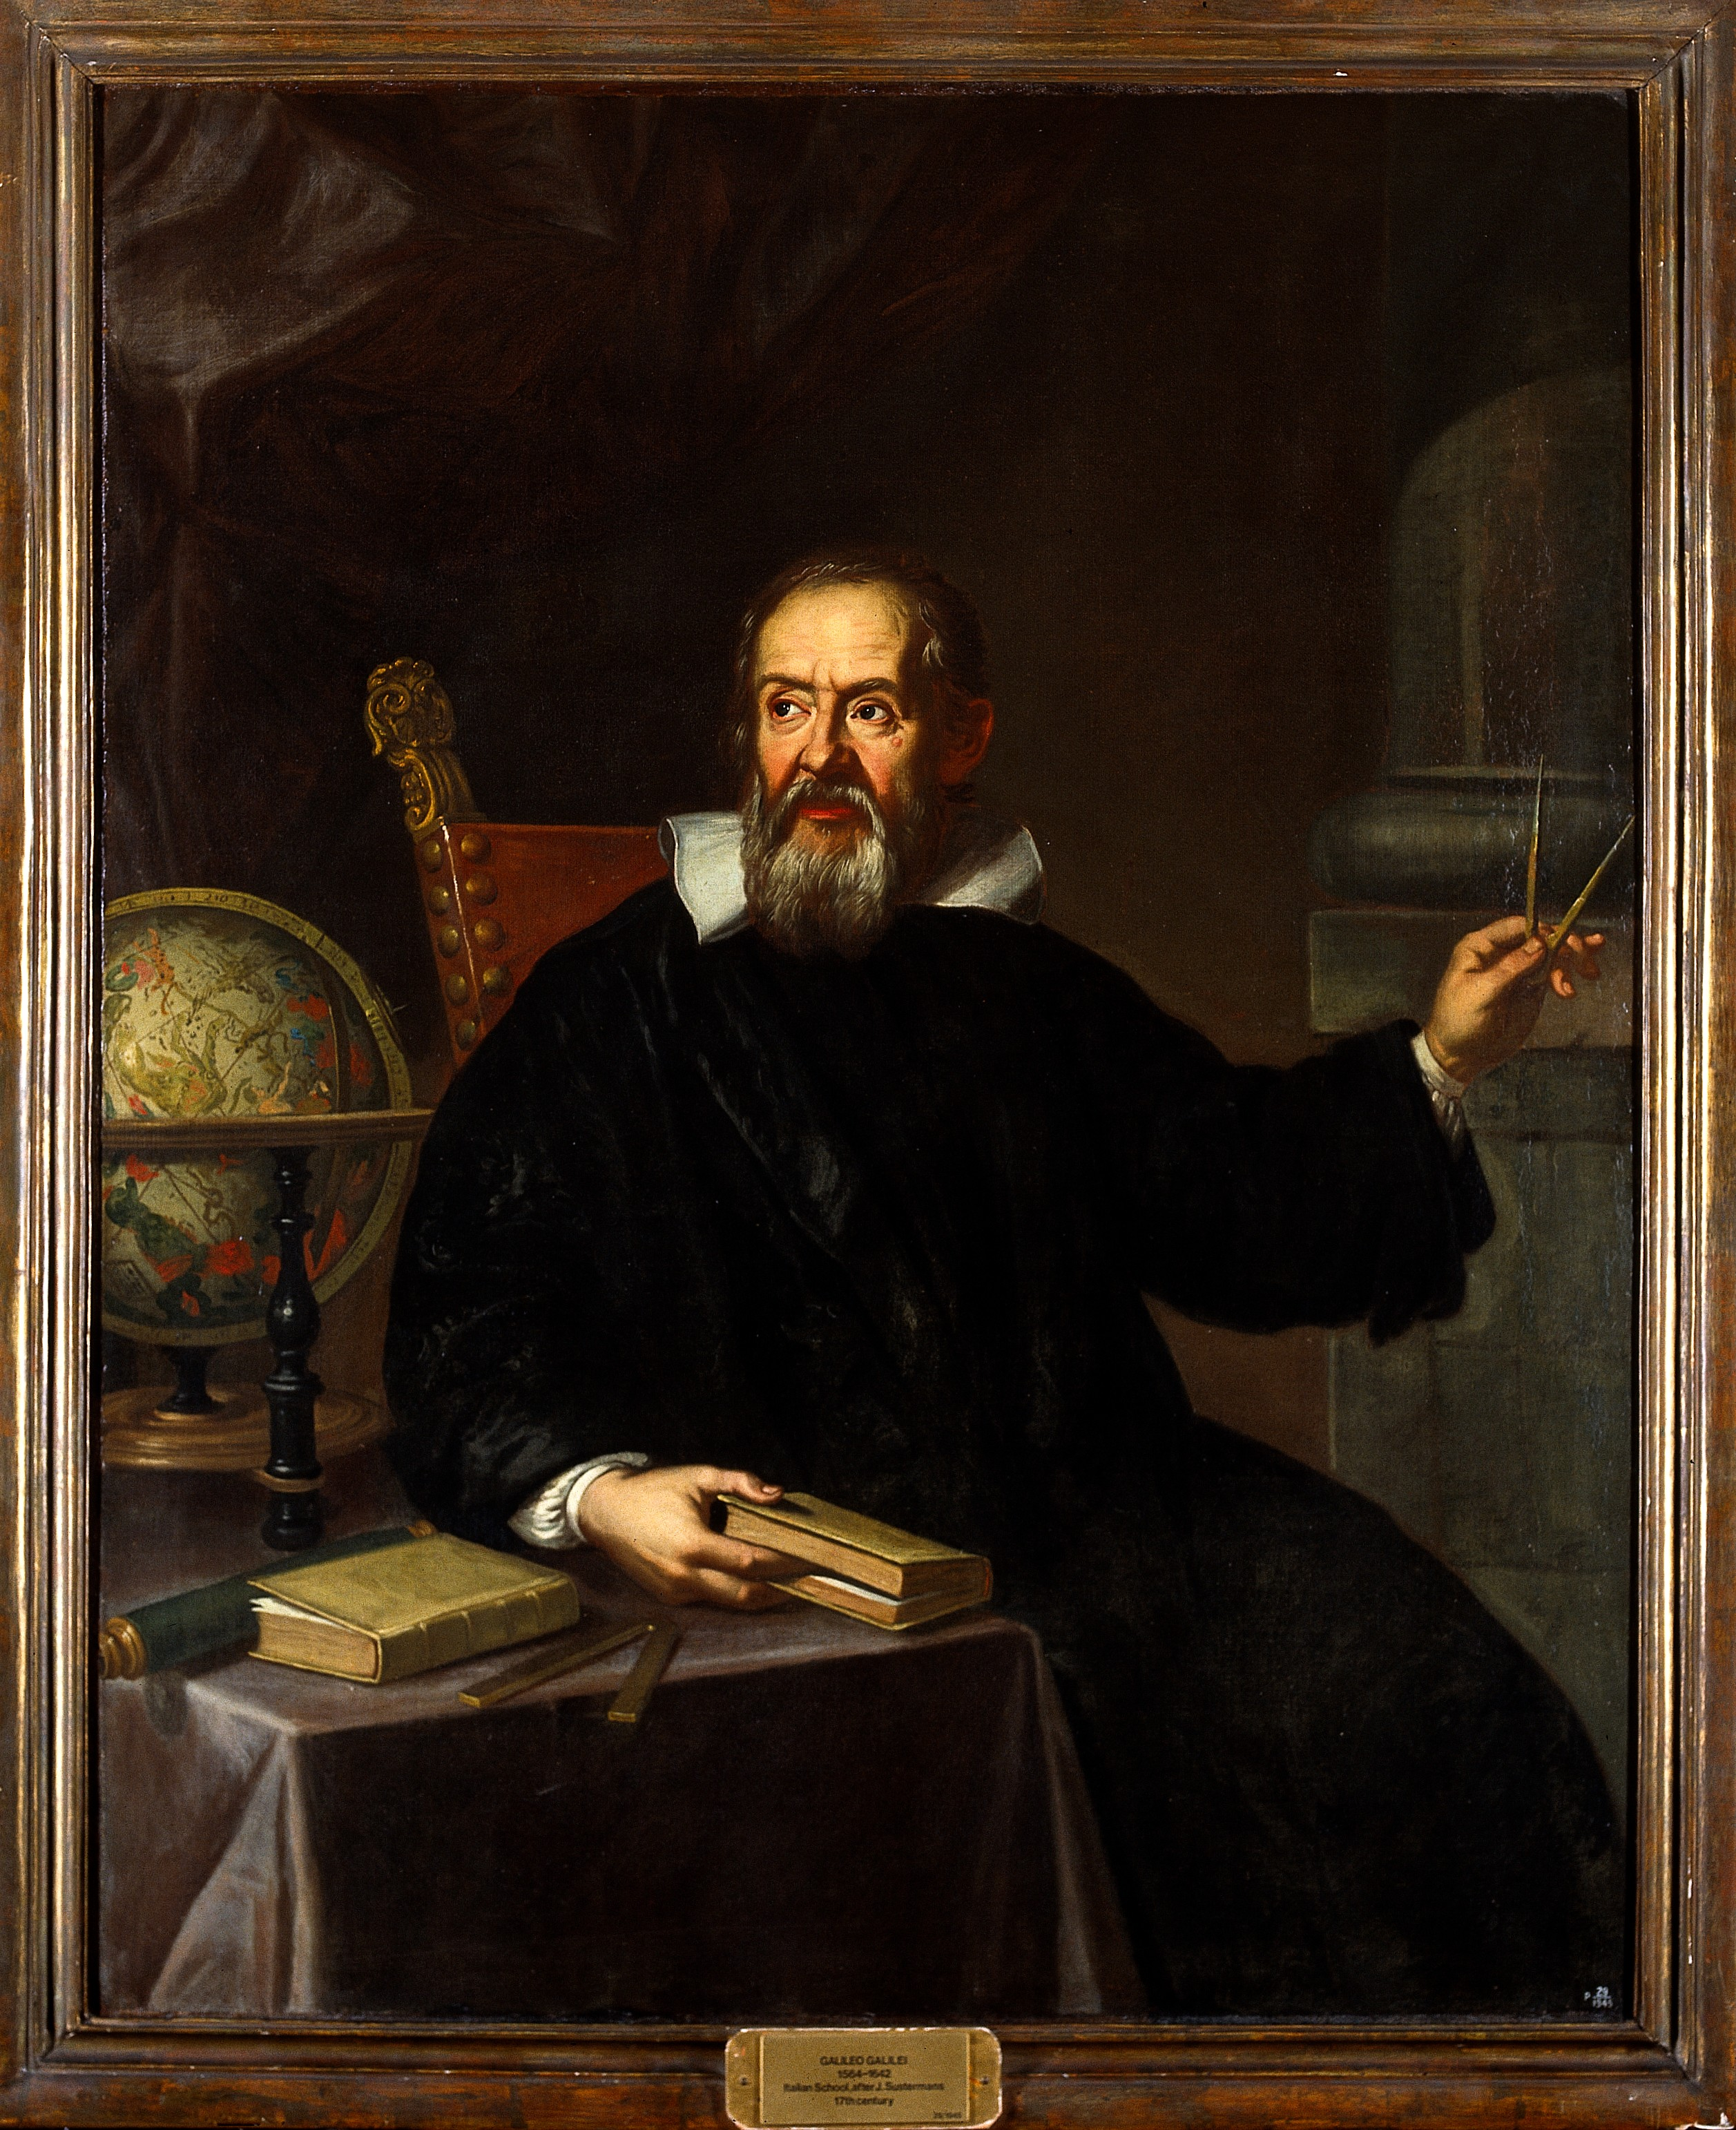
\includegraphics[width=0.7\linewidth]{images/Galileo-Galilei.jpg}
\end{figure}
\vfill

\newpage

\textit{Was du ererbt von deinen Vätern hast, Erwirb es, um es zu besitzen}

\rule{\linewidth}{0.4pt}
\begin{flushright}
\textsc{goethe}
\end{flushright}
%\noindent
\vfill
\begin{figure}[ht]
	\centering
	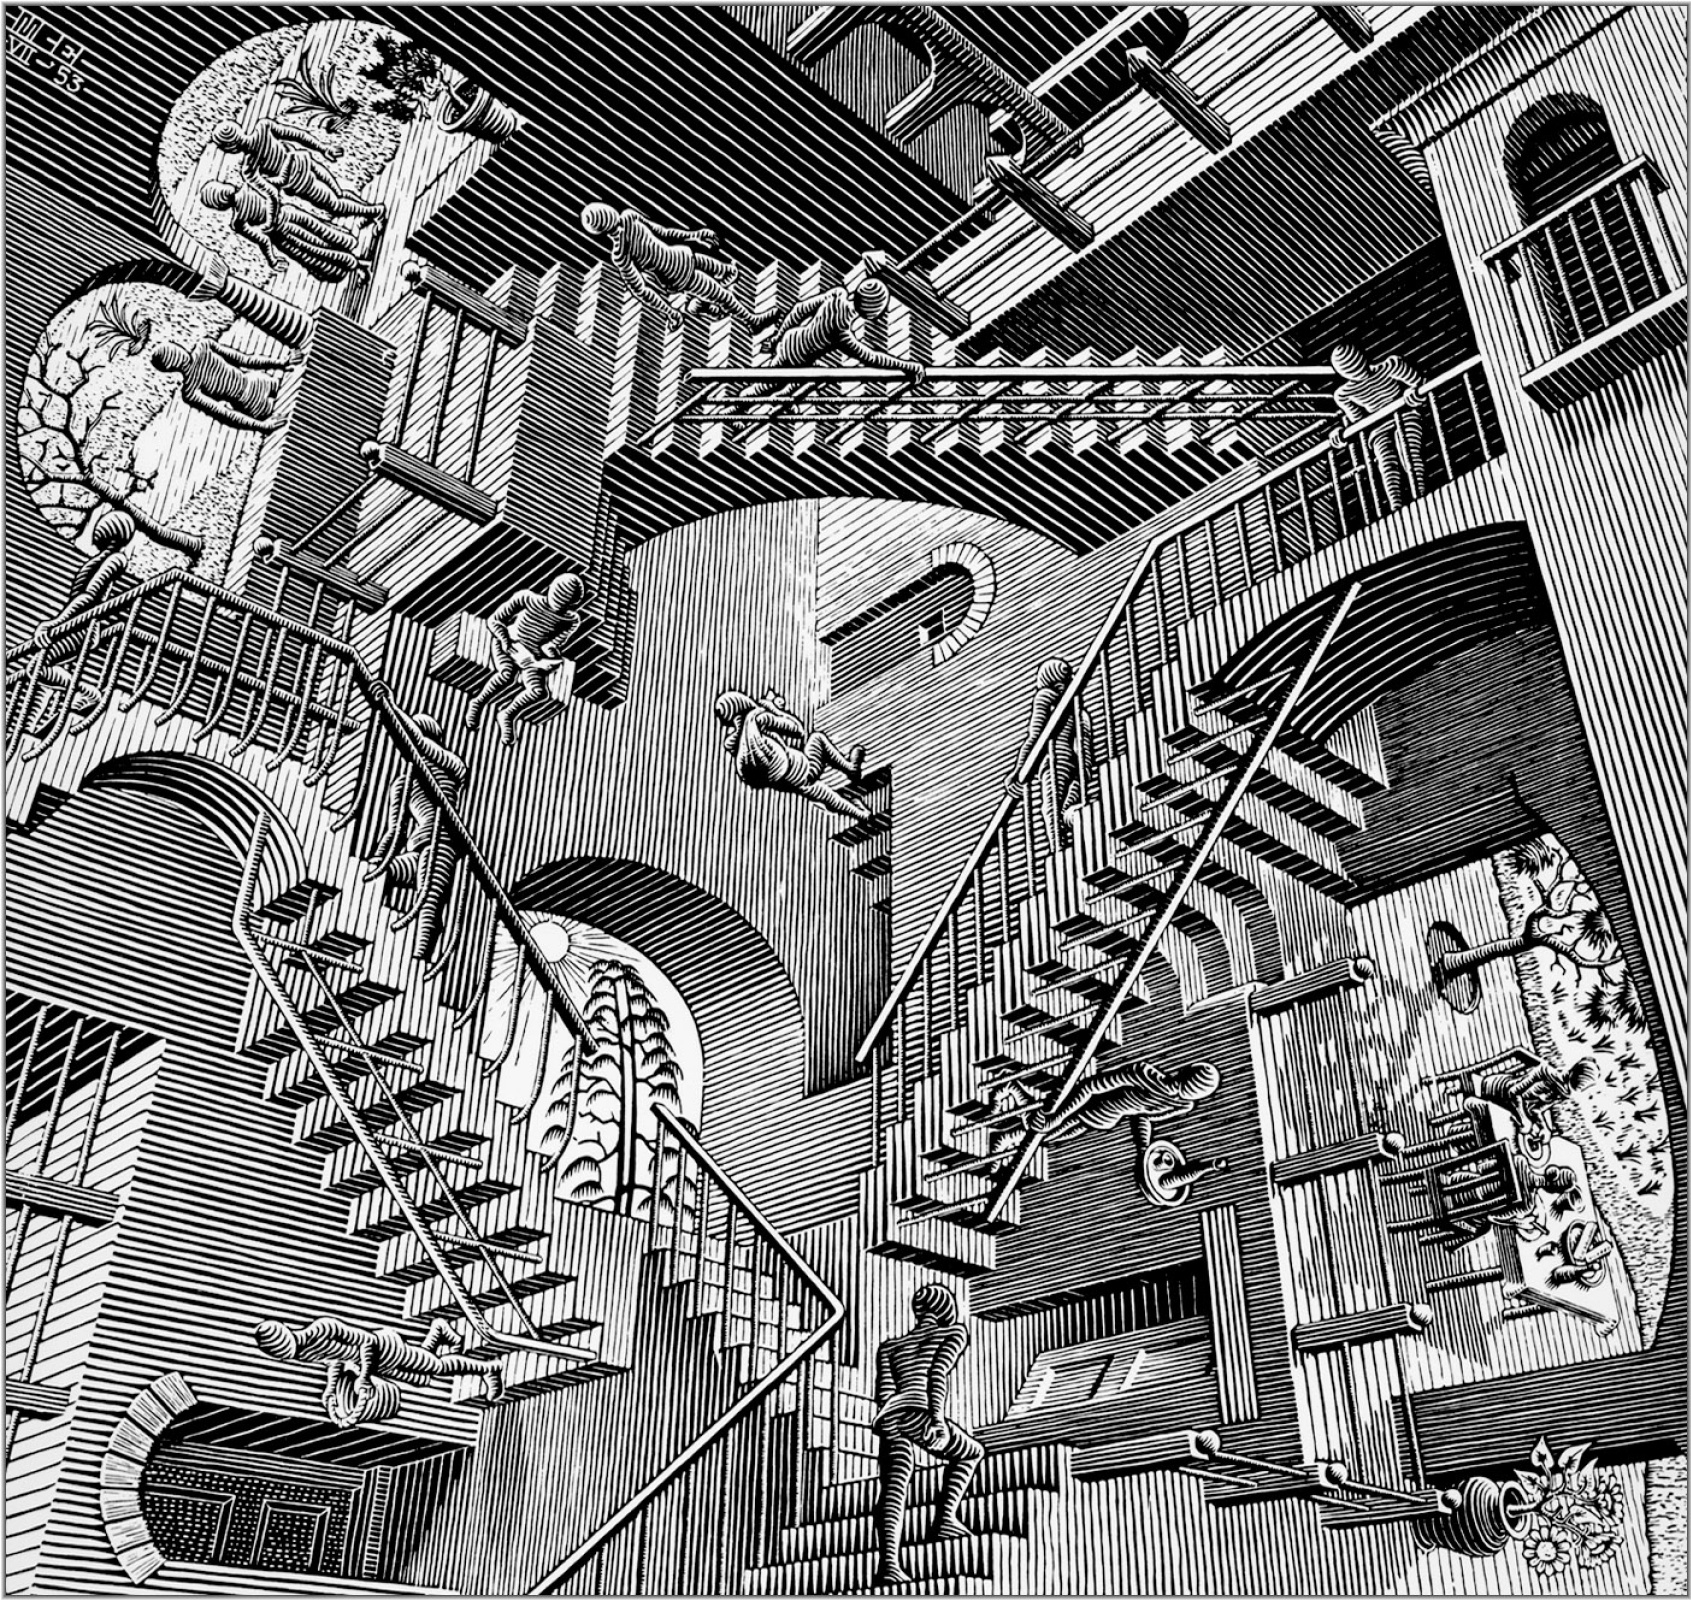
\includegraphics[width = 0.8\linewidth]{images/relatividad_escher.jpg}
	\caption{\textit{Relatividad} por M.C. Escher (1953).}
\end{figure}
\vfill

\newpage
\section{Invariance vs covariance}
We would discuss how the concepts of \textit{invariance} and \textit{covariance} are present in Classical mechanics, Special Relativity and General Relativity. We would figure it out the intrinsic relation between invariance and covariance, and how they are used in physics theories mentioned above.

\subsection*{The idea behind Equivalence Principle}
Gauss assumes that in every point of a surface is always possible to choose a cartesian system of coordinates wich satisfies euclidian geometry locally, for a small neighbourhood of the point. This idea extends to any hypersurface in the Riemmannian geometry. The initial assumption of Gauss implies that is possible to entirely know the curvature of a surface with the function of transformation of the cartesian coordinates $\xi$ to the surface coordinates $x$. This is analog to the Equivalence Principle in which is possible to determine all the effects of gravitational field in terms of the field equation of an inertial coordinate system $\xi$ extendended to a general system of coordinates $x$, by using the metric  $g_{\mu,\nu}$ and the connection $\Gamma^{\gamma}\,_{\mu \nu}$ that depends on the metric and the connection for the inertial system through the transformation rule of coordinates $\xi^\alpha(x^\mu)$.

$$\Gamma^\lambda\,_{\mu\nu} = \frac{\partial x^\lambda}{\partial \xi^\alpha}\frac{\partial^2\xi^\alpha}{\partial x^\mu \partial x^\nu}$$

$$g_{\mu\nu}=\frac{\partial \xi^\alpha}{\partial x^\mu} \frac{\partial \xi^\beta}{\partial x^\nu} \eta_{\alpha\beta}$$

We note from this the essence of the kind of invariance that is present in General Relativity, that is that when we pass to an equation valid for a local inertial system (of Special Relativity) to its form for a general system then the metric and the affine connection come up, in such a way, the new equation is a tensorial equation that preservs its structure or form under general coordinate transformations $x^\mu \to x'^\mu$.

As an example, following \cite{weinberg}, for a weak static field generated by nonrelativistic matter in a inertial system we have
\begin{equation}
	\nabla^2g_{00}=-8\pi GT_{00} \label{eq:field-intertial-system}
\end{equation}
that is obtained based on the Newtonian potential $\phi$ determined by Poisson's equation ${\nabla^2 \phi = 4\pi G \rho}$, where $\rho$ is the mass density. Equation \ref{eq:field-intertial-system} allows to guess that the field equation for the inertial system is of the form
\begin{equation}
	G_{\alpha\beta} = -8\pi GT_{\alpha\beta}
\end{equation}
where $G_{\alpha\beta}$ is a linear combination of the metric and its first and second derivates. So, from the Principle of Equivalence the equation that govern gravitational fields of arbitrary strength and in a general frame must take the form
\begin{equation}
	G_{\mu\nu} = -8\pi GT_{\mu\nu}
\end{equation}
where $G_{\mu\nu}$ is a tensor that reduces to $G_{\alpha\beta}$ for weak fields. After certain derivations that do not concern here\footnote{For a complete description see \cite{weinberg}} we get
\begin{equation}
	G_{\mu\nu} = R_{\mu\nu}-\frac{1}{2}g_{\mu\nu}R \label{eq:Guv}
\end{equation}
where $R_{\mu\nu}=R^\lambda\,_{\mu\lambda\nu}$ is the Ricci tensor and $R=R^\mu\,_\mu$ is the curvature scalar. Finally, in equation \ref{eq:Guv} we can expect to have terms related to the metric $g_{\mu\nu}$ and the affine connection $\Gamma^\lambda_{\mu\nu}$ that are not present in $G_{\alpha\beta}$ for the local inertial system. Thus, the field equation of gravity differs for a local inertial system (locally Minkowski) related to a general system by the coming up of the metric and the affine connection. On the next section we will see that the Principle of Special Relativity and the Galileo's Principle Relativity of the invariance of the law of physics are preciesly characterized by the fact that nothing comes up or disappear while changing from one inertial system to another. In the present case, equation \ref{eq:field-intertial-system} shows that at least there is one coordinate system in wich the metric becomes $\eta_{\alpha\beta}$ and the affine connection becames zero $\Gamma^\lambda\,_{\alpha\beta}=0$. We will come back to analyze this fact when we will talk about the Principle of General Covariance.

\subsection*{Galileo's Principle of Relativity}
Galileo's Principle of Relativity can be statement in the form\footnote{See for example \cite{arnold}}

\textit{There exist coordinate systems, called intertial, possesing the following properties:}
\begin{itemize}
	\item[\textit{1}] \textit{All the laws of the nature at all moments of time are the same in all inertial coordinate systems.}
	\item[\textit{2}] \textit{All coordinate systems in uniform rectilinear motion with respect to an inertial one are themselves inertial.}
\end{itemize}

Here we want to point out what it means for the laws of physics that they \textit{are the same} in all inertial coordinate systems. For this we means that the law of physics is invariant under the action of the Galileo's group, which is that the law equations keep its form under a Galilean transformation $T$ that belongs to the Galilean group $\mathscr{G}$.

The Galilean group $\mathscr{G}$ is defined as the set of invertible affine transformations of the four-dimensional affine space $A^4$ that represents the Newtonian spacetime. To belong to the Galilean group, a transformation ${T:A^4\to A^4}$ must preserve the time interval of any pair of events and preserve the distance between two simoultaneous events, that is
\begin{itemize}
	\item[1.] $\Delta  t_{pq} = \Delta t_{T(p)T(q)}
$ for any $p$ and $q$ in $A^4$.
	\item[2.] If $p$ and $q$ are in $A^4$, and $\Delta t_{pq}=0$ then $||\overrightarrow{pq}||=|| \overrightarrow{T(p)T(q)}||$
\end{itemize}

where $\Delta t_{pq}$ depends on a non-zero linear form $\tau:\Re^4\to\Re$ such that $\Delta t_{pq}:=\tau(\overrightarrow{pq})$, and $||.||$ is a norm that depends on an inner product $\left<.,.\right>$ defined on the kernel subspace of $\tau$.

There exists 10 independently transformations of this kind that are basis for the Galilean group, we clasify them in three classes
\begin{enumerate}
	\item \textsc{uniform motion with velocity} $\vec{v}$
	$$g_1((t,\vec{x}))=(t,\vec{x}+\vec{v}t)\, , \, \vec{v}\in\Re^3$$
	\item \textsc{translation of the origin $(0,0)$ to $(s,\vec{w})$}
	$$g_2((t,\vec{x}))=(t+s,\vec{x}+\vec{w})\, , \, (s,\vec{w})\in\Re\times\Re^3 $$
	\item \textsc{Rotation $R$ of the coordinate axis}
	$$g_3((t,\vec{x}))=(t,R\vec{x})\, , \, R\in SO(3,\Re)$$
\end{enumerate}

where here $(t,\vec{x})\in \Re\times\Re^3$, and $SO(n,\Re)$ holds for the special orthogonal group of $n\times n$ orthogonal matrices with determinant equals to 1 and with reals entries. The $SO(n,\Re)$ group has dimension of $n(n-1)/2$. Is left as an excersice to the read prove that this transformations belongs to the Galilean group. 

We note that a general Galilean transformation is of the form
\begin{equation}
	T(t,\vec{x})=(t+s,R\vec{x}+\vec{u}t+\vec{w})\,,\, s\in\Re\,,\,\vec{u},\vec{w}\in\Re^3\,,\,R\in SO(3,\Re) \label{eq:generalT}
\end{equation}
so acording to the Galileo's Principle of Relativity the laws of physics must remain the same under coordinate transformations $(t,\vec{x})\mapsto (t',\vec{x}')$ that in case of Newtonian physics are the Galilean transformations. This kind of invariance is that we call covariance, wich express specificly that the structure\footnote{This idea of covariance is present in all classical physics. In GR exists the Principle of General Covariance that uses this idea as is discussed in \cite{weinberg}} of the equation remains the same. For clarify this ideas we will do an example. Let's take the Newton's second law for a system of a single particle
\begin{equation}
	\vec{F}=\dot{\vec{p}} \label{eq:F = dot p}
\end{equation}

Also let's assume that the particle is inmersed in a scalar potential field $U(||\vec{r}-\vec{r}_0||)$ that depends only in the distance relative to some point $\vec{r}_0$. So that the Newton's second law of motion converts in
\begin{equation}
	\vec{\nabla}U(||\vec{r}-\vec{r}_0||) = \dot{\vec{p}} \label{eq:2nd Law}
\end{equation}
So now we make a coordinate transformation $\vec{r}\to\vec{r}\,'$ of the form of \ref{eq:generalT} but changing $R\to A$ for have a convenient notation. Firstly, we note that the distance ${R:=||\vec{r}-\vec{r}_0||=||\vec{r}\,'-\vec{r}\,'_0||:=R'}$ remain the same by definition of Galilean transformation. This implies that the scalar potential remain the same ${U(R)=U(R')}$. Secondlly, for the momentum we get
\begin{equation}
	\frac{d\vec{p}}{dt} = \frac{dm}{dt}\vec{v}+ m\frac{d\vec{v}}{dt} \label{eq:dpdt}
\end{equation}
Then using the assumption that $m=m'$ by experimental facts for non-relativistic physics, and as $t'=t+s$ with $s$ a constant we have
\begin{equation}
\frac{dm}{dt}=\frac{dm'}{dt'} \underbrace{\frac{dt'}{dt}}_{=1}=\frac{dm'}{dt'} \label{eq:dmdt}
\end{equation}
As $dt=dt'$ we will use the notation $\dot{\vec{a}}$ for the time derivate of a vector $\vec{a}$ indistinguishably for $t$ and $t'$. For the position vector we have
\begin{equation}
	 \vec{r}\,' = A\vec{r} + \vec{u}t+\vec{w} \label{eq:r}
\end{equation}
\begin{equation}
	\dot{\vec{r}}\,' = A\dot{\vec{r}} + \vec{u} \label{eq:dotr}
\end{equation}
\begin{equation}
	\ddot{\vec{r}}\,' = A\ddot{\vec{r}} \label{eq:ddotr}
\end{equation}
Therefore replacing \ref{eq:dmdt}, \ref{eq:dotr}, and \ref{eq:ddotr} in \ref{eq:dpdt} we obtain
$$	\frac{d\vec{p}}{dt} = \frac{dm'}{dt'}A^{-1}(\vec{v}\,'-\vec{u}) + m'A^{-1} \frac{d\vec{v}\,'}{dt'} $$ 
\begin{equation}
	\frac{d\vec{p}}{dt} = A^{-1}\left( \frac{d\vec{p}\,'}{dt'}-\frac{dm'}{dt'}\vec{u}\right) \label{eq: t dpdt}
\end{equation}
We recall that $A^{-1}$ always exists as each orthogonal matrix has determinant distinct to zero. Thirdly, we focus on the gradient operator $\vec{\nabla}$ acting on $U$. Let us recall that $U$ depends only on the distance $||\vec{r}-\vec{r}_0||=R$, then from vector calculus we know
\begin{equation}
	\vec{\nabla}U(R)=\frac{\partial U}{\partial R}\hat{R}=\frac{\partial U}{\partial R'}\underbrace{\frac{\partial R'}{\partial R}}_{=1} \hat{R}
\end{equation}
\begin{equation}
	\vec{\nabla}U(R) = \frac{\partial U}{\partial R'} \frac{\vec{r}-\vec{r}_0}{|| \vec{r}-\vec{r}_0 ||} \label{eq:grad U}
\end{equation}
Equation \ref{eq:r} holds for every position vector $\vec{r}$ in $\Re^3$, in particular it holds for $\vec{r}_0$
\begin{equation}
	\vec{r}\,'_0 = A \vec{r}_0+\vec{u}t+\vec{w}
\end{equation}
And so, using \ref{eq:r}
\begin{equation}
	\vec{r}\,'-\vec{r}\,'_0 = A(\vec{r}-\vec{r'})
\end{equation}
Then, equation \ref{eq:grad U} can be written as
\begin{equation}
	\vec{\nabla} U(R)  = \frac{\partial  U}{\partial R'} A^{-1} \frac{\vec{r}\,'-\vec{r}\,'_0}{|| \vec{r}\,'-\vec{r}\,'_0 ||} = A^{-1} \frac{\partial U(R')}{\partial R'} \hat{R}'=A^{-1}\vec{\nabla}\,'U(R') \label{eq:t nabla U}
\end{equation}
Finally, by equations \ref{eq:t nabla U} and \ref{eq: t dpdt} the Newton's second law \ref{eq:2nd Law} transform as
\begin{equation}
	A^{-1}\vec{\nabla}\,'U(R') = A^{-1}\left( \frac{d\vec{p}\,'}{dt'}-\frac{dm'}{dt'}\vec{u}\right)
\end{equation}
Multiplying the matrix $A$ by left in both sides of equations we have
\begin{equation}
	\vec{\nabla}\,'U(R') = \left( \frac{d\vec{p}\,'}{dt'}-\frac{dm'}{dt'}\vec{u}\right)
\end{equation}

By assuming that the particle do not change its mass $dm' / dt'=0$ and by noting that $\vec{\nabla}\,'U(R')$ is the force in the transformated frame we obtain
\begin{equation}
	\vec{F}\,' = \dot{\vec{p}}\,' \label{eq: F' = dot p'}
\end{equation}

We can see that the equation \ref{eq: F' = dot p'} keep his form under Galilean transformations, and equally important, it is completely determined by quantities of its own reference frame. It do not involves variables related to another inertial frame, as for example its relative velocity  or relative orientation of axes to some other reference frame. In fact, when we develope a Galilean transformation of coordinates $(t,\vec{r})\mapsto (t',\vec{r}\,')$

\subsection*{Lorentz's Invariance}
\subsection*{Principle of General Covariance}

\bibliography{References.bib}
\bibliographystyle{unsrt}

\end{document}